\documentclass[conference]{IEEEtran}
\usepackage[T1]{fontenc}
\usepackage[english,spanish,es-tabla]{babel}
\usepackage{graphicx}
\usepackage{booktabs}
\usepackage{pifont}
\usepackage{cite}
\usepackage{url}
\usepackage{xcolor}

\graphicspath{{../figures/}}
% Colocación de flotantes más permisiva: el artículo tiene 13 tablas y figuras
\renewcommand{\topfraction}{0.9}
\renewcommand{\dbltopfraction}{0.9}
\renewcommand{\textfraction}{0.1}
\renewcommand{\floatpagefraction}{0.8}
\renewcommand{\dblfloatpagefraction}{0.8}
\setcounter{topnumber}{3}
\setcounter{dbltopnumber}{3}
\setlength{\textfloatsep}{12pt plus 2pt minus 2pt}
\setlength{\dbltextfloatsep}{12pt plus 2pt minus 2pt}
\newcommand{\todo}[1]{\textcolor{red}{[#1]}}
\newcommand{\bien}{\ding{51}}
\newcommand{\mal}{\ding{55}}
\newcommand{\gc}[1]{\includegraphics[width=0.1\textwidth]{gradcam/#1.png}}

\begin{document}
\bstctlcite{IEEEexample:BSTcontrol}

\title{Comparación de ResNet50, EfficientNet-B0 y Swin-T para la clasificación de lesiones cutáneas en ISIC 2019 bajo un protocolo común}

\author{\IEEEauthorblockN{Santiago Valdés Uriarte}
\IEEEauthorblockA{Maestría en Inteligencia Artificial y Ciencia de Datos\\
Universidad Panamericana\\
Aguascalientes, México\\
\todo{correo}}}

\maketitle

\begin{abstract}
Las comparaciones entre redes convolucionales y Transformers para dermatoscopia suelen usar particiones, resoluciones y métricas distintas, y sus cifras no se pueden contrastar entre sí. En este trabajo se comparan ResNet50, EfficientNet-B0 y Swin-T en ISIC 2019 (ocho clases, 25,331 imágenes) con un protocolo único: partición 70/15/15 agrupada por lesión, los mismos hiperparámetros para los tres modelos, tres semillas y el test oficial del reto sin la clase UNK (6,191 imágenes) como evaluación externa. Swin-T obtiene el mejor F1 macro en el test interno, 58.9~$\pm$~1.5, contra 53.2~$\pm$~0.5 de EfficientNet-B0 y 52.0~$\pm$~1.4 de ResNet50, y conserva el orden en el test oficial (58.5). EfficientNet-B0 requiere 0.4 GMACs por imagen y procesa 3,096 imágenes por segundo, y el promedio de tres de sus semillas llega a 56.7. Quitar la ponderación de clases sube la exactitud, pero baja la exactitud balanceada de ResNet50 de 58.4 a 48.7. Grad-CAM produce mapas comparables en las dos CNN y artefactos de ventana en Swin-T.
\end{abstract}

\renewcommand{\IEEEkeywordsname}{Palabras clave}
\begin{IEEEkeywords}
clasificación de lesiones cutáneas, ISIC 2019, redes convolucionales, Swin Transformer, desbalance de clases, Grad-CAM, costo computacional.
\end{IEEEkeywords}

\begin{otherlanguage}{english}
\begin{abstract}
Comparisons between convolutional networks and Transformers for dermoscopy usually rely on different splits, resolutions and metrics, so their figures cannot be contrasted. This work compares ResNet50, EfficientNet-B0 and Swin-T on ISIC 2019 (eight classes, 25,331 images) under a single protocol: a 70/15/15 split grouped by lesion, the same hyperparameters for the three models, three seeds, and the official challenge test set without the UNK class (6,191 images) as external evaluation. Swin-T achieves the best macro F1 on the internal test set, 58.9~$\pm$~1.5, against 53.2~$\pm$~0.5 for EfficientNet-B0 and 52.0~$\pm$~1.4 for ResNet50, and keeps the ranking on the official test set (58.5). EfficientNet-B0 needs 0.4 GMACs per image and processes 3,096 images per second, and averaging three of its seeds reaches 56.7. Removing class weighting raises accuracy but lowers the balanced accuracy of ResNet50 from 58.4 to 48.7. Grad-CAM yields comparable maps for both CNNs and window artifacts for Swin-T.
\end{abstract}
\renewcommand{\IEEEkeywordsname}{Index Terms}
\begin{IEEEkeywords}
skin lesion classification, ISIC 2019, convolutional neural networks, Swin Transformer, class imbalance, Grad-CAM, computational cost.
\end{IEEEkeywords}
\end{otherlanguage}

\section{Introducción}

La clasificación automática de lesiones cutáneas con redes convolucionales tomó otra escala cuando Esteva et al.~\cite{esteva2017dermatologist} mostraron que una Inception v3 alcanzaba un desempeño comparable al de dermatólogos en tareas binarias. Dos años después, en el estudio internacional sobre el reto ISIC 2018, los algoritmos superaron en promedio a los lectores humanos, aunque la ventaja se redujo con imágenes fuera de la distribución de entrenamiento~\cite{tschandl2019comparison}. Ese matiz es el punto de partida de este trabajo: el desempeño que se reporta de un clasificador depende tanto de la arquitectura como de las condiciones en que se evalúa.

Las cifras publicadas sobre ISIC 2019 ilustran el problema: van de 74.2 de exactitud balanceada para el ganador del reto~\cite{gessert2020isic} a 91.87 de exactitud para modelos tipo Swin~\cite{aruk2026comparison,ayas2023swin}, pero cada trabajo usa su propia partición, resolución, datos y métrica, y ninguna de esas cifras se puede poner junto a otra. A esto se suman dos riesgos documentados. Cassidy et al.~\cite{cassidy2022isic} encontraron imágenes duplicadas dentro de cada edición de ISIC y entre ediciones, que inflan las métricas cuando la partición no agrupa por lesión, y Daneshjou et al.~\cite{daneshjou2022disparities} mostraron que modelos de dermatología de última generación pierden mucho desempeño en un conjunto externo con tonos de piel diversos y enfermedades poco comunes.

En este artículo comparo ResNet50, EfficientNet-B0 y Swin-T con un protocolo fijo que atiende esos dos riesgos y que se aplica igual a las tres arquitecturas. La partición agrupa las imágenes por lesión, los hiperparámetros son los mismos, cada modelo se entrena con tres semillas y la evaluación externa usa el test oficial de ISIC 2019, que nunca interviene en una decisión de entrenamiento. El costo se mide en una sola GPU de laptop y la interpretabilidad con Grad-CAM sobre las mismas imágenes para los tres modelos. El objetivo no es alcanzar el estado del arte, sino saber cómo se ordenan las arquitecturas con un presupuesto fijo: imágenes de 224 píxeles, 15 épocas y 12~GB de VRAM.

Swin-T resulta el mejor modelo por 5.7 puntos porcentuales (pp) de F1 macro, y EfficientNet-B0 el de mejor relación entre costo y desempeño. Dos experimentos complementarios, uno con el doble de épocas y otro que cambia la ponderación de clases, no alteran ese orden, y el segundo descarta la hipótesis que motivó correrlo.

\section{Trabajo relacionado}

ResNet~\cite{he2016resnet} y EfficientNet~\cite{tan2019efficientnet} son las dos familias convolucionales más usadas como base en dermatoscopia. ResNet introdujo las conexiones residuales que permiten entrenar redes profundas, y EfficientNet escala de forma conjunta la profundidad, el ancho y la resolución de la red. El ganador de ISIC 2019 combinó EfficientNets de varias resoluciones con SENet y ResNeXt, una pérdida balanceada, data augmentation fuerte y la metadata del paciente~\cite{gessert2020isic}. Ese tipo de ensemble grande es el estándar de los retos, y es también lo que hace difícil aislar el aporte de cada arquitectura.

Del lado de los Transformers, ViT trata la imagen como una secuencia de parches con atención global~\cite{dosovitskiy2021vit}, mientras que Swin agrega una jerarquía de cuatro etapas y restringe la atención a ventanas locales que se desplazan entre capas~\cite{liu2021swin}. Shamshad et al.~\cite{shamshad2023transformers} revisan su adopción en imagen médica. La referencia más directa para este trabajo es la de Matsoukas et al.~\cite{matsoukas2021replace,matsoukas2023pretrained}, que comparan ResNet50 con DeiT-S bajo un mismo protocolo en tres conjuntos médicos, uno de ellos ISIC 2019. Desde cero ganan las CNN por mucho; con pesos de ImageNet la brecha desaparece (en ISIC 2019, recall de 0.810 para ResNet50 contra 0.844 para DeiT-S, mediana de cinco repeticiones), y con preentrenamiento autosupervisado los ViT ganan por poco. Raghu et al.~\cite{raghu2019transfusion} explican por qué los pesos de ImageNet ayudan aun cuando el dominio médico es distinto: más por la inicialización y la escala de los pesos que por la reutilización de características.

El trabajo más cercano a este es el de Aruk et al.~\cite{aruk2026comparison}, que compara 15 CNN y 15 ViT en HAM10000 e ISIC 2019 bajo las mismas condiciones y concluye que los modelos tipo Swin obtienen la mejor exactitud, con más parámetros y cómputo que las CNN. Ayas~\cite{ayas2023swin} llega a una conclusión parecida con un solo Swin en ISIC 2019. Frente a esos trabajos, aquí se reportan tres semillas con su desviación, la partición agrupa por lesión para evitar los duplicados que documentan Cassidy et al.~\cite{cassidy2022isic}, se agrega una evaluación externa, el costo se mide en hardware de consumo y Grad-CAM se aplica a las mismas imágenes en las tres arquitecturas. El protocolo de entrenamiento es cercano al de Matsoukas et al., que también redimensionan a 256 píxeles y usan Adam con una tasa de aprendizaje de $10^{-4}$.

\section{Metodología}

\subsection{Datos y partición}

ISIC 2019 reúne 25,331 imágenes dermatoscópicas de entrenamiento provenientes de HAM10000~\cite{tschandl2018ham10000}, BCN20000~\cite{hernandezperez2024bcn20000,combalia2019bcn20000} y el conjunto MSK~\cite{codella2017isic,codella2019isic2018}, etiquetadas en ocho clases: melanoma (MEL), nevo melanocítico (NV), carcinoma basocelular (BCC), queratosis actínica (AK), queratosis benigna (BKL), dermatofibroma (DF), lesión vascular (VASC) y carcinoma escamocelular (SCC). La clase UNK no tiene imágenes en el conjunto de entrenamiento. El desbalance es fuerte: NV concentra el 50.8\% de las imágenes y DF el 0.9\%, una razón de 54 a 1 en la partición de entrenamiento.

La partición se hizo con StratifiedGroupKFold de scikit-learn en 20 pliegues (14 para entrenamiento, 3 para validación y 3 para test, semilla 42), con \texttt{lesion\_id} como grupo. De las 25,331 imágenes, 23,247 (91.8\%) tienen \texttt{lesion\_id} y corresponden a 11,847 lesiones; las 2,084 restantes forman cada una su propio grupo. Resultan 17,735 imágenes de entrenamiento, 3,798 de validación y 3,798 de test interno, con la proporción de clases intacta y sin ninguna lesión repartida entre dos particiones. El test oficial del reto tiene 8,238 imágenes; al excluir las 2,047 etiquetadas como UNK quedan 6,191, con una mezcla de clases distinta: NV baja a 40.3\%, MEL sube a 21.4\% y AK a 6.0\%. Las particiones son las mismas en todas las corridas.

\subsection{Preprocesamiento y data augmentation}

Todas las imágenes, de entrenamiento y del test oficial, se redimensionaron una sola vez a $256\times256$ píxeles con interpolación bicúbica y se guardaron como JPEG con calidad 95. El redimensionamiento es directo, sin recorte, y deforma las imágenes de $600\times450$ píxeles; la deformación afecta por igual a los tres modelos. En entrenamiento se aplica RandomResizedCrop a 224 con escala de 0.7 a 1.0, volteo horizontal y vertical, rotación de hasta 20 grados y ColorJitter de 0.1 en brillo y contraste. En validación y test solo se toma el recorte central de 224. La normalización usa la media y la desviación de ImageNet. Para el desbalance se usa cross-entropy ponderada con pesos inversamente proporcionales a la frecuencia de cada clase en entrenamiento, normalizados a media 1, sin oversampling.

\subsection{Modelos}

Los tres modelos se tomaron de timm (\texttt{resnet50}, \texttt{efficientnet\_\allowbreak b0} y \texttt{swin\_tiny\_\allowbreak patch4\_\allowbreak window7\_\allowbreak 224}) con pesos preentrenados en ImageNet; se reemplazó la cabeza por una capa de ocho salidas y se hizo fine-tuning de la red completa. ResNet50~\cite{he2016resnet} apila bloques residuales con cuello de botella. EfficientNet-B0~\cite{tan2019efficientnet} es el modelo base de su familia, construido con bloques MBConv. Swin-T~\cite{liu2021swin} calcula la atención en ventanas de $7\times7$ parches que se desplazan entre capas consecutivas, en cuatro etapas que reducen la resolución. Sus parámetros y su costo aparecen en la Tabla~\ref{tab:costo}.

\subsection{Protocolo de entrenamiento}

Los tres modelos se entrenaron con AdamW~\cite{loshchilov2019adamw}, tasa de aprendizaje de $10^{-4}$ y weight decay de $10^{-2}$, con un warmup lineal durante la primera época y decaimiento cosine hasta el final de la época 15. El batch es de 32 imágenes y el máximo de 15 épocas, con early stopping de paciencia 3 sobre el F1 macro de validación; se conserva el checkpoint con el mejor valor. El entrenamiento usa precisión mixta en bf16, y cada modelo se corre con las semillas 0, 1 y 2, para un total de nueve corridas. Los hiperparámetros son idénticos para las tres arquitecturas por diseño; sus consecuencias se discuten en la Sección~\ref{sec:discusion}.

Después de ver las primeras corridas se decidieron dos experimentos complementarios, ambos con la semilla 0 y con el resto del protocolo intacto. En el primero, motivado por que cuatro de las primeras cinco corridas llegaron al tope de 15 épocas sin activar el early stopping, los modelos se entrenan de nuevo desde ImageNet con un máximo de 30 épocas; el cosine se ajusta a 30 épocas, así que no es una continuación de la corrida de 15. El segundo es una ablación que compara la ponderación por frecuencia inversa del protocolo con su raíz cuadrada (también normalizada a media 1) y con cross-entropy sin pesos. La hipótesis quedó escrita antes de correrla: que la ponderación inversa sube el recall de las clases raras a costa de su precisión y deprime el F1 macro. Ninguno de los dos experimentos sustituye a las nueve corridas principales.

\subsection{Métricas y protocolo de evaluación}

Cada corrida se evalúa con su mejor checkpoint en el test interno y en el test oficial. Se reportan exactitud, F1 macro (la métrica principal y la que guía el early stopping), F1 ponderado, exactitud balanceada (el recall macro), AUROC macro uno contra el resto, F1 por clase y matriz de confusión, como media y desviación estándar muestral entre las tres semillas. El test interno es la evaluación principal; el test oficial funciona como evaluación externa y no se usó para elegir ningún hiperparámetro ni checkpoint. Para medir la brecha de generalización se calcula también el F1 macro en entrenamiento con el mejor checkpoint y el transform de validación, sin augmentation.

El costo incluye los parámetros contados con torchinfo, los GMACs por imagen a 224 píxeles calculados con fvcore (lo que la literatura suele reportar como FLOPs), la VRAM pico de entrenamiento, los segundos por época sin contar la primera y el throughput de inferencia con batch 32 en bf16 sobre tensores sintéticos, es decir, sin el costo de leer las imágenes. Los ensembles promedian las probabilidades softmax ya guardadas, sin entrenar nada adicional: uno combina las tres arquitecturas con la semilla 0 y otros dos promedian las tres semillas de una misma arquitectura, como control.

\subsection{Interpretabilidad}

Los mapas de Grad-CAM~\cite{selvaraju2017gradcam} se calcularon con la biblioteca pytorch-grad-cam y la clase real como objetivo. Las capas objetivo son el último bloque de \texttt{layer4} en ResNet50, \texttt{conv\_head} en EfficientNet-B0 y la normalización final en Swin-T, con un reshape de los tokens a una rejilla de $7\times7$. Se usan 16 imágenes del test interno elegidas al azar, dos por clase: una bien clasificada y una mal clasificada por ResNet50 con la semilla 0. Las mismas 16 imágenes se usan para los otros dos modelos, también con su semilla 0.

\subsection{Entorno de cómputo}

Todo se corrió en una laptop Lenovo Legion Pro 7i con una GPU RTX 5070 Ti Laptop de 12~GB (arquitectura Blackwell), un procesador Intel Core Ultra 9 275HX y Ubuntu sobre WSL2 con 23~GiB de RAM asignados. El software es PyTorch 2.11.0 con CUDA 12.8 y timm 1.0.30. El código, las configuraciones y las particiones están en el repositorio del proyecto \todo{URL del repositorio}.

\section{Resultados}

\begin{table}[!t]
\centering
\caption{Resultados en el test interno y en el test oficial ISIC 2019 (sin UNK), en porcentaje}
\label{tab:resultados}
\footnotesize
\setlength{\tabcolsep}{4pt}
\begin{tabular}{lccc}
\toprule
Métrica & ResNet50 & EfficientNet-B0 & Swin-T \\
\midrule
\multicolumn{4}{@{}l}{Test interno (3,798 imágenes)} \\
F1 macro & 52.0 $\pm$ 1.4 & 53.2 $\pm$ 0.5 & \textbf{58.9 $\pm$ 1.5} \\
F1 ponderado & 67.1 $\pm$ 0.3 & 68.9 $\pm$ 0.2 & \textbf{73.4 $\pm$ 0.7} \\
Exact. balanceada & 56.6 $\pm$ 1.7 & 54.1 $\pm$ 0.9 & \textbf{57.7 $\pm$ 0.9} \\
Exactitud & 65.6 $\pm$ 0.4 & 68.4 $\pm$ 0.3 & \textbf{73.4 $\pm$ 0.8} \\
AUROC & 90.7 $\pm$ 0.6 & 91.8 $\pm$ 0.1 & \textbf{94.2 $\pm$ 0.2} \\
\midrule
\multicolumn{4}{@{}l}{Test oficial (6,191 imágenes)} \\
F1 macro & 51.6 $\pm$ 0.9 & 53.0 $\pm$ 1.2 & \textbf{58.5 $\pm$ 1.5} \\
Exact. balanceada & 52.8 $\pm$ 1.1 & 52.4 $\pm$ 2.1 & \textbf{55.6 $\pm$ 1.7} \\
\bottomrule
\end{tabular}
\par\vspace{2pt}
\parbox{\columnwidth}{\scriptsize Media $\pm$ desviación estándar muestral entre las semillas 0, 1 y 2. Exact. balanceada: exactitud balanceada (recall macro). AUROC macro uno contra el resto. En el test oficial se excluyeron 2,047 imágenes UNK. En negritas, la mejor media por fila.}
\end{table}

\begin{table}[!t]
\centering
\caption{F1 por clase en el test interno, en porcentaje}
\label{tab:clase}
\footnotesize
\setlength{\tabcolsep}{4pt}
\begin{tabular}{lcccc}
\toprule
Clase & ResNet50 & EfficientNet-B0 & Swin-T & Soporte \\
\midrule
MEL & 55.3 $\pm$ 0.3 & 57.7 $\pm$ 0.1 & \textbf{61.6 $\pm$ 1.6} & 678 \\
NV & 81.1 $\pm$ 0.6 & 82.1 $\pm$ 0.2 & \textbf{85.6 $\pm$ 0.4} & 1,929 \\
BCC & 60.3 $\pm$ 1.7 & 63.9 $\pm$ 0.4 & \textbf{69.1 $\pm$ 0.5} & 499 \\
AK & 34.1 $\pm$ 2.2 & \textbf{37.6 $\pm$ 2.7} & 37.0 $\pm$ 0.6 & 130 \\
BKL & 49.9 $\pm$ 0.3 & 53.2 $\pm$ 0.8 & \textbf{62.3 $\pm$ 1.0} & 394 \\
DF & 39.7 $\pm$ 6.6 & 37.0 $\pm$ 5.3 & \textbf{44.1 $\pm$ 5.8} & 36 \\
VASC & 62.9 $\pm$ 1.7 & 64.6 $\pm$ 1.4 & \textbf{71.0 $\pm$ 9.0} & 38 \\
SCC & 33.1 $\pm$ 2.6 & 29.3 $\pm$ 3.9 & \textbf{40.5 $\pm$ 2.8} & 94 \\
\bottomrule
\end{tabular}
\par\vspace{2pt}
\parbox{\columnwidth}{\scriptsize Media $\pm$ desviación estándar muestral entre las semillas 0, 1 y 2. En negritas, el mejor modelo por clase. Soporte: imágenes de cada clase en el test interno. MEL: melanoma; NV: nevo melanocítico; BCC: carcinoma basocelular; AK: queratosis actínica; BKL: queratosis benigna; DF: dermatofibroma; VASC: lesión vascular; SCC: carcinoma escamocelular.}
\end{table}

\begin{figure*}[!t]
\centering
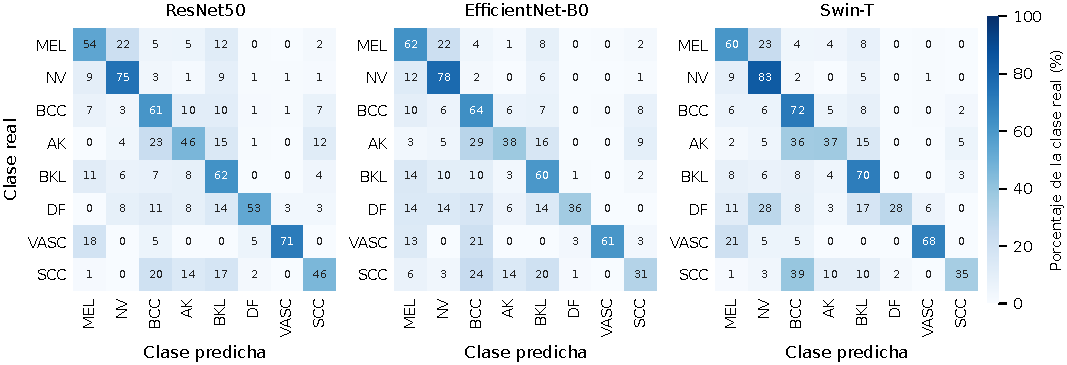
\includegraphics[width=\textwidth]{fig3_matrices_confusion.pdf}
\caption{Matrices de confusión en el test interno con la semilla 0 de cada modelo, en porcentaje de cada clase real (las filas suman 100). Siglas de las clases como en la Tabla~\ref{tab:clase}.}
\label{fig:confusion}
\end{figure*}

\begin{figure*}[!t]
\centering
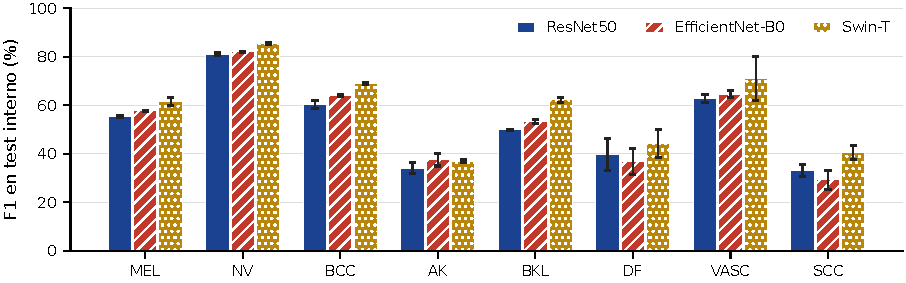
\includegraphics[width=0.85\textwidth]{fig4_f1_por_clase.pdf}
\caption{F1 por clase en el test interno (media de las semillas 0, 1 y 2; las barras de error marcan una desviación estándar). Las barras más largas, en DF y en VASC de Swin-T, corresponden a clases con 36 y 38 imágenes.}
\label{fig:clase}
\end{figure*}

\subsection{Desempeño}

Swin-T tiene la mejor media en todas las métricas y en los dos conjuntos de evaluación (Tabla~\ref{tab:resultados}). Su F1 macro en el test interno es de 58.9~$\pm$~1.5, contra 53.2~$\pm$~0.5 de EfficientNet-B0 y 52.0~$\pm$~1.4 de ResNet50, y su AUROC de 94.2 contra 91.8 y 90.7. Entre las dos CNN el orden depende de la métrica. EfficientNet-B0 queda arriba en F1 macro y en exactitud, mientras que ResNet50 lo supera en exactitud balanceada (56.6 contra 54.1).

Por clase, Swin-T es el mejor en siete de las ocho (Tabla~\ref{tab:clase} y Figura~\ref{fig:clase}); la excepción es AK, donde EfficientNet-B0 obtiene 37.6 contra 37.0. Las clases más difíciles para los tres modelos son AK, SCC y DF, con F1 de 29.3 a 44.1. Las matrices de confusión de la semilla 0 (Figura~\ref{fig:confusion}) muestran de dónde viene buena parte del error: entre 23 y 36\% de las AK y entre 20 y 39\% de los SCC se clasifican como BCC, y entre 22 y 23\% de los MEL como NV. En Swin-T, el 28\% de los DF termina en NV.

\begin{table}[!t]
\centering
\caption{Costo computacional en una RTX 5070 Ti Laptop (12 GB), entrada de $224\times224$}
\label{tab:costo}
\footnotesize
\setlength{\tabcolsep}{4pt}
\begin{tabular}{lccc}
\toprule
 & ResNet50 & EfficientNet-B0 & Swin-T \\
\midrule
Parámetros (M) & 23.5 & \textbf{4.0} & 27.5 \\
GMACs & 4.1 & \textbf{0.4} & 4.5 \\
s/época & 36.3 $\pm$ 2.9 & \textbf{25.4 $\pm$ 1.7} & 46.1 $\pm$ 1.1 \\
Tiempo total (min) & 8.6 $\pm$ 1.8 & \textbf{6.9 $\pm$ 0.4} & 11.0 $\pm$ 1.0 \\
VRAM pico (GiB) & 1.8 & \textbf{1.4} & 2.6 \\
Inferencia (img/s) & 1,770 & \textbf{3,096} & 1,189 \\
Época del mejor F1 val. & 10.7 $\pm$ 2.5 & 12.3 $\pm$ 0.6 & 13.0 $\pm$ 2.6 \\
\bottomrule
\end{tabular}
\par\vspace{2pt}
\parbox{\columnwidth}{\scriptsize GMACs: miles de millones de multiplicaciones-acumulaciones por imagen (fvcore). s/época: entrenamiento más validación, desde la época 2. Tiempo total: todas las épocas hasta el early stopping. Medición descrita en la Sección~III-E. Media $\pm$ desviación estándar entre semillas. En negritas, el menor costo.}
\end{table}

\begin{figure}[!t]
\centering
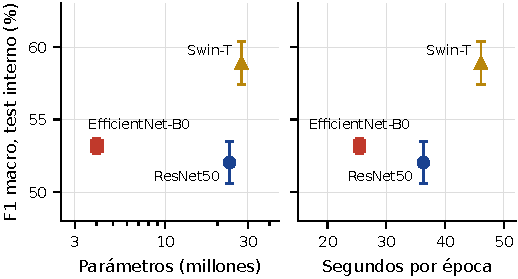
\includegraphics[width=\columnwidth]{fig5_f1_vs_costo.pdf}
\caption{F1 macro en el test interno contra el número de parámetros (escala logarítmica) y contra los segundos por época. Las barras marcan una desviación estándar entre semillas.}
\label{fig:costo}
\end{figure}

\subsection{Costo computacional}

EfficientNet-B0 es el más ligero en todos los ejes de la Tabla~\ref{tab:costo}: tiene la sexta parte de los parámetros de ResNet50 y menos de la décima parte de sus GMACs, y en inferencia procesa 3,096 imágenes por segundo, contra 1,770 de ResNet50 y 1,189 de Swin-T (Figura~\ref{fig:costo}). Ninguno se acerca al límite de la tarjeta: la VRAM pico va de 1.4 a 2.6~GiB con batch 32, y una corrida completa tarda en promedio entre 6.9 y 11.0 minutos.

\subsection{Convergencia}

Las curvas de validación (Figura~\ref{fig:curvas}) separan a Swin-T desde la primera época, con un F1 macro de 38.7 contra 31.4 de EfficientNet-B0 y 26.3 de ResNet50. En la época 5, Swin-T (54.3) ya supera el mejor valor medio que ResNet50 alcanza en las 15 épocas (52.2). En promedio, la mejor época fue la 10.7 para ResNet50, la 12.3 para EfficientNet-B0 y la 13.0 para Swin-T (Tabla~\ref{tab:costo}). El early stopping solo se activó en tres de las nueve corridas, dos de ResNet50 y una de Swin-T; ninguna de EfficientNet-B0 se detuvo antes del tope, y las otras dos semillas de Swin-T tuvieron su mejor época en la 14 y la 15.

\begin{figure}[!t]
\centering
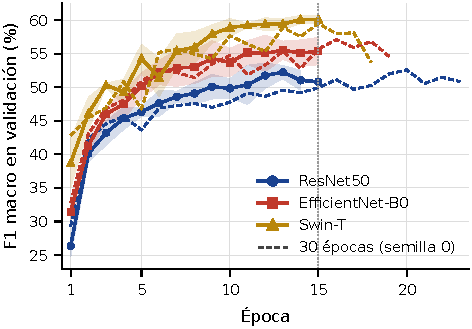
\includegraphics[width=0.9\columnwidth]{fig1_curvas_val.pdf}
\caption{F1 macro de validación por época. Líneas continuas: media de las semillas 0, 1 y 2 con 15 épocas (la banda marca una desviación estándar; en las últimas épocas la media incluye solo las semillas que siguen corriendo). Líneas punteadas: semilla 0 con un máximo de 30 épocas.}
\label{fig:curvas}
\end{figure}

\begin{table}[!t]
\centering
\caption{Experimento de convergencia: máximo de 15 contra 30 épocas (semilla 0)}
\label{tab:convergencia}
\footnotesize
\setlength{\tabcolsep}{2.5pt}
\begin{tabular}{lcccccccc}
\toprule
 & \multicolumn{2}{c}{Época} & \multicolumn{3}{c}{F1 interno} & \multicolumn{3}{c}{F1 oficial} \\
\cmidrule(lr){2-3} \cmidrule(lr){4-6} \cmidrule(lr){7-9}
Modelo & 15 & 30 & 15 & 30 & $\Delta$ & 15 & 30 & $\Delta$ \\
\midrule
ResNet50 & 13/15 & 20/23 & 53.5 & 54.0 & +0.5 & 51.9 & 53.0 & +1.1 \\
EfficientNet-B0 & 13/15 & 16/19 & 53.6 & 54.7 & +1.1 & 51.7 & 52.7 & +1.0 \\
Swin-T & 10/13 & 15/18 & 57.2 & 60.3 & +3.1 & 57.9 & 59.1 & +1.2 \\
\bottomrule
\end{tabular}
\par\vspace{2pt}
\parbox{\columnwidth}{\scriptsize Época: época del mejor F1 macro de validación / épocas corridas hasta el early stopping (paciencia 3). F1 macro en porcentaje; $\Delta$ en puntos porcentuales. Con una sola semilla, $\Delta$ se compara con la desviación entre semillas de la Tabla~\ref{tab:resultados}.}
\end{table}

Con un máximo de 30 épocas (Tabla~\ref{tab:convergencia}), el early stopping cortó en las épocas 23, 19 y 18, con la mejor época en la 20, la 16 y la 15. El F1 macro del test interno subió 0.5~pp en ResNet50, 1.1 en EfficientNet-B0 y 3.1 en Swin-T, y el del test oficial 1.1, 1.0 y 1.2~pp.

\begin{figure}[!t]
\centering
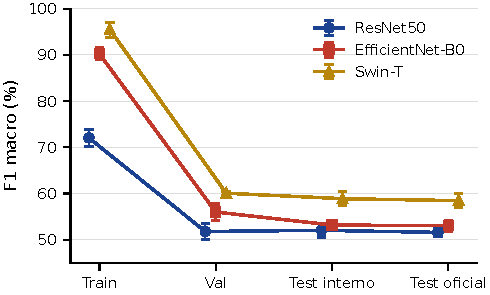
\includegraphics[width=\columnwidth]{fig6_brecha_generalizacion.pdf}
\caption{F1 macro en entrenamiento (mejor checkpoint, sin augmentation), validación, test interno y test oficial. Media y desviación estándar de las semillas 0, 1 y 2.}
\label{fig:brecha}
\end{figure}

\subsection{Generalización}

En entrenamiento, ResNet50 llega a 72.0 de F1 macro, EfficientNet-B0 a 90.2 y Swin-T a 95.5, contra 51.8, 56.0 y 60.1 en validación, con brechas de 20, 34 y 35~pp (Figura~\ref{fig:brecha}). Del test interno al oficial, el F1 macro cae 0.4, 0.2 y 0.4~pp, menos que la desviación entre semillas de cada modelo. Las otras métricas sí caen: la exactitud balanceada 3.8, 1.7 y 2.1~pp; la exactitud 3.5, 4.0 y 4.3~pp (de 65.6 a 62.1, de 68.4 a 64.4 y de 73.4 a 69.1), y el AUROC 2.5, 2.6 y 2.2~pp (de 90.7 a 88.2, de 91.8 a 89.2 y de 94.2 a 92.0). El F1 de DF se mueve en sentido contrario y sube en el test oficial: de 39.7 a 48.1 en ResNet50, de 37.0 a 48.6 en EfficientNet-B0 y de 44.1 a 60.8 en Swin-T.

\begin{table}[!t]
\centering
\caption{Ensembles por promedio de probabilidades softmax, F1 macro y exactitud balanceada en porcentaje}
\label{tab:ensembles}
\footnotesize
\setlength{\tabcolsep}{2pt}
\begin{tabular}{lcccc}
\toprule
 & \multicolumn{2}{c}{Test interno} & \multicolumn{2}{c}{Test oficial} \\
\cmidrule(lr){2-3} \cmidrule(lr){4-5}
 & F1 & Exact. bal. & F1 & Exact. bal. \\
\midrule
Swin-T (media) & 58.9 $\pm$ 1.5 & 57.7 $\pm$ 0.9 & 58.5 $\pm$ 1.5 & 55.6 $\pm$ 1.7 \\
EfficientNet-B0 (media) & 53.2 $\pm$ 0.5 & 54.1 $\pm$ 0.9 & 53.0 $\pm$ 1.2 & 52.4 $\pm$ 2.1 \\
\midrule
Arquitecturas (semilla 0) & 59.3 & \textbf{58.8} & 58.2 & 56.6 \\
Semillas Swin-T & \textbf{60.5} & 58.5 & \textbf{60.5} & \textbf{57.0} \\
Semillas EfficientNet-B0 & 56.7 & 56.8 & 56.9 & 55.6 \\
\bottomrule
\end{tabular}
\par\vspace{2pt}
\parbox{\columnwidth}{\scriptsize Arquitecturas: ResNet50, EfficientNet-B0 y Swin-T con semilla 0. Semillas: las semillas 0, 1 y 2 de una misma arquitectura (control). Las filas de media son modelos individuales, con su desviación estándar entre semillas.}
\end{table}

\subsection{Ensembles}

El ensemble de las tres arquitecturas con semilla 0 obtiene 59.3 de F1 macro en el test interno y 58.2 en el oficial (Tabla~\ref{tab:ensembles}). El de las tres semillas de Swin-T llega a 60.5 en ambos, y el de las tres semillas de EfficientNet-B0 a 56.7 y 56.9, 3.5 y 3.9~pp sobre la media individual de ese modelo. La comparación del ensemble de arquitecturas depende de contra qué Swin-T se mida. Usa la semilla 0, la más débil de las tres (57.2), y frente a ella gana 2.1~pp, pero frente a la media de Swin-T gana 0.4 en el test interno y pierde 0.3 en el oficial.

\begin{table*}[!t]
\centering
\caption{Ablación de la ponderación de clases en la pérdida (semilla 0), en porcentaje}
\label{tab:ablacion}
\footnotesize
\setlength{\tabcolsep}{3pt}
\begin{tabular}{lccccccccc}
\toprule
 &  & \multicolumn{2}{c}{Test interno} & \multicolumn{2}{c}{Test oficial} & \multicolumn{4}{c}{Clases minoritarias, test interno} \\
\cmidrule(lr){3-4} \cmidrule(lr){5-6} \cmidrule(lr){7-10}
Modelo & Ponderación & F1 macro & Exact. bal. & F1 macro & Exact. bal. & DF (P / R) & VASC (P / R) & SCC (P / R) & AK (P / R) \\
\midrule
ResNet50 & Frecuencia inversa & 53.5 & \textbf{58.4} & \textbf{51.9} & \textbf{53.2} & 40.4 / 52.8 & 58.7 / 71.1 & 29.3 / 45.7 & 26.8 / 46.2 \\
 & Raíz cuadrada & \textbf{53.9} & 54.8 & 51.5 & 50.2 & 27.9 / 33.3 & 68.6 / 63.2 & 35.1 / 36.2 & 36.0 / 49.2 \\
 & Sin pesos & 52.5 & 48.7 & 46.6 & 43.7 & 75.0 / 16.7 & 90.9 / 52.6 & 26.2 / 18.1 & 38.8 / 34.6 \\
\midrule
EfficientNet-B0 & Frecuencia inversa & \textbf{53.6} & \textbf{53.6} & \textbf{51.7} & 50.0 & 50.0 / 36.1 & 65.7 / 60.5 & 25.7 / 30.9 & 40.8 / 37.7 \\
 & Raíz cuadrada & 51.8 & 51.7 & \textbf{51.7} & \textbf{50.6} & 33.3 / 22.2 & 66.7 / 63.2 & 29.3 / 38.3 & 36.8 / 30.0 \\
 & Sin pesos & 51.6 & 49.2 & 51.0 & 48.4 & 38.9 / 19.4 & 72.4 / 55.3 & 33.3 / 27.7 & 39.4 / 28.5 \\
\midrule
Swin-T & Frecuencia inversa & 57.2 & 56.7 & \textbf{57.9} & \textbf{55.7} & 62.5 / 27.8 & 60.5 / 68.4 & 49.3 / 35.1 & 36.1 / 36.9 \\
 & Raíz cuadrada & \textbf{59.9} & \textbf{57.8} & 56.7 & 53.7 & 50.0 / 33.3 & 68.6 / 63.2 & 61.8 / 36.2 & 41.7 / 36.9 \\
 & Sin pesos & 56.5 & 53.3 & 56.6 & 53.1 & 66.7 / 22.2 & 79.3 / 60.5 & 46.4 / 34.0 & 35.0 / 33.1 \\
\bottomrule
\end{tabular}
\par\vspace{2pt}
\parbox{\textwidth}{\scriptsize Frecuencia inversa: pesos $1/n$ (protocolo principal). Raíz cuadrada: $1/\sqrt{n}$. Ambos normalizados a media 1. Sin pesos: cross-entropy estándar. P / R: precisión / recall. En negritas, la mejor variante de cada modelo por columna de métrica global.}
\end{table*}

\begin{figure}[!t]
\centering
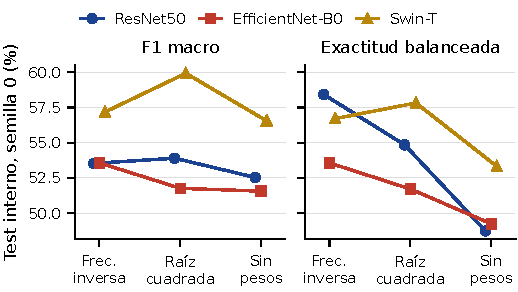
\includegraphics[width=\columnwidth]{fig7_ablacion_pesos.pdf}
\caption{F1 macro y exactitud balanceada en el test interno según la ponderación de clases (semilla 0). El F1 macro casi no cambia entre variantes, mientras que la exactitud balanceada cae al quitar los pesos en los tres modelos.}
\label{fig:ablacion}
\end{figure}

\subsection{Ablación de la ponderación de clases}

Al quitar los pesos (Tabla~\ref{tab:ablacion} y Figura~\ref{fig:ablacion}), la exactitud sube en los tres modelos (en ResNet50, de 65.9 a 72.7) y la exactitud balanceada baja (de 58.4 a 48.7, de 53.6 a 49.2 y de 56.7 a 53.3), mientras que el F1 macro apenas cae 1.0, 2.0 y 0.7~pp; en el test oficial, ResNet50 sin pesos baja a 46.6 de F1 macro. Las clases minoritarias muestran el mecanismo: sin pesos, ResNet50 tiene en DF una precisión de 75.0 y un recall de 16.7, contra 40.4 y 52.8 con frecuencia inversa.

\begin{figure*}[!t]
\centering
\scriptsize
\setlength{\tabcolsep}{1pt}
\renewcommand{\arraystretch}{0.9}
\begin{tabular}{@{}r*{8}{c}@{}}
 & MEL (mal) & NV (bien) & BCC (mal) & AK (bien) & BKL (mal) & DF (bien) & VASC (mal) & SCC (bien) \\
\raisebox{0.045\textwidth}{\rotatebox{90}{Original}} & \gc{ISIC_0025800_original} & \gc{ISIC_0003462_downsampled_original} & \gc{ISIC_0057336_original} & \gc{ISIC_0056073_original} & \gc{ISIC_0026607_original} & \gc{ISIC_0069930_original} & \gc{ISIC_0061674_original} & \gc{ISIC_0025811_original} \\
\raisebox{0.045\textwidth}{\rotatebox{90}{ResNet50}} & \gc{ISIC_0025800_resnet50} & \gc{ISIC_0003462_downsampled_resnet50} & \gc{ISIC_0057336_resnet50} & \gc{ISIC_0056073_resnet50} & \gc{ISIC_0026607_resnet50} & \gc{ISIC_0069930_resnet50} & \gc{ISIC_0061674_resnet50} & \gc{ISIC_0025811_resnet50} \\
 & SCC \mal & NV \bien & MEL \mal & AK \bien & SCC \mal & DF \bien & MEL \mal & SCC \bien \\
\raisebox{0.02\textwidth}{\rotatebox{90}{EfficientNet-B0}} & \gc{ISIC_0025800_efficientnet_b0} & \gc{ISIC_0003462_downsampled_efficientnet_b0} & \gc{ISIC_0057336_efficientnet_b0} & \gc{ISIC_0056073_efficientnet_b0} & \gc{ISIC_0026607_efficientnet_b0} & \gc{ISIC_0069930_efficientnet_b0} & \gc{ISIC_0061674_efficientnet_b0} & \gc{ISIC_0025811_efficientnet_b0} \\
 & SCC \mal & NV \bien & MEL \mal & AK \bien & NV \mal & BKL \mal & BCC \mal & SCC \bien \\
\raisebox{0.045\textwidth}{\rotatebox{90}{Swin-T}} & \gc{ISIC_0025800_swin_t} & \gc{ISIC_0003462_downsampled_swin_t} & \gc{ISIC_0057336_swin_t} & \gc{ISIC_0056073_swin_t} & \gc{ISIC_0026607_swin_t} & \gc{ISIC_0069930_swin_t} & \gc{ISIC_0061674_swin_t} & \gc{ISIC_0025811_swin_t} \\
 & MEL \bien & NV \bien & MEL \mal & BCC \mal & BCC \mal & BKL \mal & MEL \mal & AK \mal \\
\end{tabular}
\caption{Grad-CAM con la clase real como objetivo (semilla 0 de cada modelo) en ocho imágenes del test interno, una por clase. Encabezado: clase real y si ResNet50 la clasificó bien o mal. Debajo de cada mapa, la clase predicha por ese modelo (\bien: correcta, \mal: incorrecta). Imágenes, de izquierda a derecha: ISIC\_0025800, ISIC\_0003462, ISIC\_0057336, ISIC\_0056073, ISIC\_0026607, ISIC\_0069930, ISIC\_0061674 e ISIC\_0025811. Las otras ocho imágenes del conjunto fijo están en el repositorio como material complementario.}
\label{fig:gradcam}
\end{figure*}

\subsection{Interpretabilidad}

La Figura~\ref{fig:gradcam} muestra ocho de las 16 imágenes, una por clase, alternando casos bien y mal clasificados por ResNet50. En las dos CNN los mapas se concentran sobre la lesión en la mayoría de los casos. En Swin-T aparecen en bloques, con patrones en cruz que siguen la partición en ventanas, y a menudo cubren el fondo: en el NV, que los tres modelos clasifican bien, el mapa de Swin-T se extiende por casi toda la imagen sin destacar la lesión. En el BKL, el mapa de ResNet50 solo se activa en una esquina y el de Swin-T sale vacío, y en el DF el de EfficientNet-B0 dibuja un anillo alrededor de la lesión sin cubrirla.

\section{Discusión}
\label{sec:discusion}

Swin-T es el mejor de los tres modelos con un margen que no depende de la semilla. Su ventaja de 5.7~pp de F1 macro sobre EfficientNet-B0 equivale a casi cuatro veces la desviación más alta entre semillas (1.5), y el margen supera esa desviación en todas las métricas salvo una: en exactitud balanceada interna, frente a ResNet50, la diferencia es de 1.1~pp con una desviación de 1.7. El resultado coincide con lo que reportan Matsoukas et al.~\cite{matsoukas2021replace} con pesos de ImageNet y con Aruk et al.~\cite{aruk2026comparison} y Ayas~\cite{ayas2023swin}, que ubican a Swin como el mejor en ISIC 2019. Este estudio no aísla el mecanismo detrás de esa ventaja, pues compara un solo Transformer contra dos CNN bajo un protocolo fijo.

Con el costo, la recomendación cambia: EfficientNet-B0 requiere menos de la décima parte de los MACs de Swin-T (0.4 contra 4.5 GMACs) y procesa 2.6 veces más imágenes por segundo, a cambio de 5.7~pp de F1 macro (Figura~\ref{fig:costo}). ResNet50, en cambio, queda dominado: EfficientNet-B0 lo supera en F1 macro, exactitud y AUROC con menos parámetros, menos cómputo, menos memoria y menos tiempo por época. La única métrica en la que ResNet50 queda arriba es la exactitud balanceada (56.6 contra 54.1 en el test interno y 52.8 contra 52.4 en el oficial), y en el oficial esa diferencia es menor que la desviación entre semillas.

ResNet50 está subajustado. Su F1 macro en entrenamiento es de 72.0, contra 90.2 de EfficientNet-B0 y 95.5 de Swin-T (Figura~\ref{fig:brecha}), y su brecha menor entre entrenamiento y validación (20~pp contra 34 y 35) se debe a que aprende menos y no a que generalice mejor. La corrida de 30 épocas apunta en la misma dirección, pues su mejor época fue la 20. Considero que la causa más probable es la tasa de aprendizaje compartida de $10^{-4}$, que para una ResNet50 con fine-tuning completo puede quedarse corta, aunque no lo probé. El protocolo común es justo en condiciones, pero no pone a cada arquitectura en su mejor configuración. Esto es una limitación de este estudio y de la mayoría de los comparativos, incluidos los de Matsoukas et al. y Aruk et al.

Los ensembles indican que promediar ayuda más cuando los modelos son parecidos en calidad. El de arquitecturas no supera al de semillas de Swin-T (59.3 contra 60.5) y en el test oficial queda por debajo de Swin-T sola: las dos CNN, más débiles, diluyen al mejor modelo. En el otro extremo, tres EfficientNet-B0 promediados llegan a 56.7 con 1.2 GMACs en total, por encima de un ResNet50 solo (52.0 con 4.1 GMACs). Frente a los ensembles grandes que ganan los retos~\cite{gessert2020isic}, varios modelos chicos promediados son una alternativa razonable cuando el costo de inferencia importa.

La evaluación externa confirma el orden, pero no todas las métricas responden igual al cambio de conjunto. El F1 macro casi no se mueve (0.2 a 0.4~pp), mientras que la exactitud balanceada, la exactitud y el AUROC caen entre 1.7 y 4.3~pp. Parte de la explicación está en la mezcla de clases del test oficial (Sección~III-A): con menos NV (40.3 contra 50.8\%), la clase en la que los tres modelos aciertan más, la exactitud global baja. La mezcla no explica la caída de la exactitud balanceada ni la del AUROC, que no dependen de la proporción de clases, así que en el test oficial los modelos sí reconocen peor cada clase. Mi lectura es que el F1 macro se sostiene porque la precisión de las clases minoritarias mejora cuando son más frecuentes y compensa la pérdida de recall; es consistente con que el F1 de DF, con 91 imágenes en el oficial contra 36 en el interno, suba en los tres modelos, aunque no medí la precisión por clase en ese conjunto. El F1 macro resulta la métrica que menos delata el cambio de conjunto y conviene leerlo junto con la exactitud balanceada. La caída es moderada frente a la que documentan Daneshjou et al.~\cite{daneshjou2022disparities} y no altera el orden entre arquitecturas.

La ablación descarta la hipótesis que la motivó. Si la ponderación inversa deprimiera el F1 macro, suavizarla o quitarla debería subirlo, y no ocurre: sin pesos el F1 baja en los tres modelos, y con la raíz cuadrada cambia en direcciones opuestas (+0.4, \textminus1.8 y +2.7~pp). En Swin-T, el 59.9 de la raíz cuadrada iguala a la mejor de sus tres semillas con frecuencia inversa, así que no se distingue del efecto de la semilla. Lo que sí cambia de forma consistente es la exactitud balanceada (Figura~\ref{fig:ablacion}): sin pesos se desploma (ResNet50 pasa de 58.4 a 48.7) mientras la exactitud sube, porque el modelo predice cada vez menos las clases raras. La frecuencia inversa es la mejor o empata en F1 macro del test oficial en los tres modelos (Tabla~\ref{tab:ablacion}) y es la mejor en exactitud balanceada en cuatro de las seis comparaciones. El mecanismo que suponía la hipótesis existe, ya que con pesos el recall de las clases raras sube y su precisión baja, pero los dos efectos se compensan en el F1. El F1 macro bajo de este estudio no se explica por la intensidad de la ponderación.

Quince épocas dejan algo sin aprovechar, pero no cambian el orden. Con 30 épocas las ganancias van de 0.5 a 3.1~pp en el test interno, y la mayor, la de Swin-T, se explica en parte por la semilla: la semilla 0 era la más débil de las tres (57.2), y el 60.3 que alcanza con 30 épocas queda 1.4~pp sobre la media de sus tres semillas con 15, dentro de la desviación de 1.5. Swin-T rinde más por época, pero cada época le cuesta 46.1~s contra 36.3 de ResNet50 y 25.4 de EfficientNet-B0.

Grad-CAM permite comparar las dos CNN entre sí, pero no a las CNN con Swin-T. En Swin-T los mapas heredan la geometría de las ventanas, y algunos salen vacíos porque, cuando el gradiente hacia la clase real es negativo en toda la capa, el ReLU de Grad-CAM lo anula. A eso se suma que la capa objetivo de Swin-T es una normalización y no una convolución, mientras que el método se diseñó para mapas convolucionales~\cite{selvaraju2017gradcam}. Matsoukas et al.~\cite{matsoukas2021replace} argumentan que los mapas de atención de un Transformer son más finos que los de Grad-CAM en una CNN, y los artefactos que aparecen aquí al forzar Grad-CAM en Swin-T son consistentes con esa idea. Lo reporto como una limitación del método: en el NV de la Figura~\ref{fig:gradcam}, Swin-T acierta con un mapa que no destaca la lesión, lo que dice más sobre Grad-CAM que sobre lo que el modelo usa para decidir.

El nivel absoluto de los tres modelos está por debajo de lo publicado. La exactitud va de 65.6 a 73.4, contra 91.87 de Aruk et al.~\cite{aruk2026comparison}, y la exactitud balanceada de 54.1 a 57.7, contra 74.2 de Gessert et al.~\cite{gessert2020isic} y 82.3 de Ayas~\cite{ayas2023swin}. Las particiones son distintas y esas cifras no se comparan directamente, pero la distancia es demasiado grande para atribuirla solo a eso. Las causas probables son varias: imágenes de 224 píxeles, data augmentation suave, 15 épocas, una partición estricta por lesión que impide que una misma lesión aparezca en entrenamiento y test~\cite{cassidy2022isic}, el redimensionamiento que deforma las imágenes de $600\times450$, y la ausencia de test-time augmentation, de metadata y de ensembles grandes. Ninguna de esas decisiones favorece a una arquitectura sobre otra.

La variabilidad entre semillas limita lo que se puede afirmar sobre las clases minoritarias. DF y VASC tienen 36 y 38 imágenes en el test interno, así que un solo acierto más en DF mueve su recall 2.8~pp. La desviación del F1 de DF va de 5.3 a 6.6~pp en los tres modelos y la de VASC llega a 9.0 en Swin-T (Tabla~\ref{tab:clase}); con esos márgenes, las diferencias entre modelos en esas clases no se interpretan. Tres semillas son el mínimo para reportar una desviación, y los experimentos de una sola semilla (convergencia, ablación y ensemble de arquitecturas) se leen con la misma reserva.

\section{Conclusiones y trabajo futuro}

Para quien tenga que clasificar lesiones con un presupuesto parecido al de este estudio, con imágenes de 224 píxeles, pocas épocas y una GPU de laptop, la elección depende de cuánto pese el costo de inferencia. Si el desempeño es lo primero y el cómputo no limita, Swin-T es la opción, y su ventaja se sostiene fuera de la partición interna. Si el modelo tiene que correr en hardware modesto o atender muchas imágenes por segundo, EfficientNet-B0 es el punto de partida, y promediar varias de sus semillas cierra buena parte de la distancia con Swin-T sin acercarse a su costo. Con la configuración compartida de este estudio no hay un escenario en el que ResNet50 convenga; queda abierto si una tasa de aprendizaje ajustada a la arquitectura cambiaría esa conclusión. En cuanto a la ponderación de clases, la frecuencia inversa es un valor por defecto razonable cuando importa no perder las clases raras.

El trabajo futuro sale de las limitaciones. Lo primero es ajustar los hiperparámetros por arquitectura, empezando por la tasa de aprendizaje de ResNet50, para separar el efecto del protocolo del de la arquitectura. Después vienen una mayor resolución, el preentrenamiento autosupervisado, que en Matsoukas et al.~\cite{matsoukas2023pretrained} favorece a los ViT y que Shamshad et al.~\cite{shamshad2023transformers} señalan como dirección abierta en imagen médica, y la metadata del paciente, que formó parte de la solución ganadora de ISIC 2019~\cite{gessert2020isic}. Para la interpretabilidad de Swin-T, attention rollout~\cite{abnar2020attention} es una alternativa más acorde con su arquitectura que Grad-CAM.

\section*{Agradecimientos}

Este trabajo usa el conjunto ISIC 2019, distribuido bajo la licencia CC-BY-NC 4.0, sin fines comerciales. BCN\_20000 Dataset: (c) Department of Dermatology, Hospital Clínic de Barcelona. HAM10000 Dataset: (c) by ViDIR Group, Department of Dermatology, Medical University of Vienna; \url{https://doi.org/10.1038/sdata.2018.161}. MSK Dataset: (c) Anonymous; \url{https://arxiv.org/abs/1710.05006}; \url{https://arxiv.org/abs/1902.03368}.

El código y el borrador del texto se desarrollaron con asistencia de Claude (Anthropic) bajo mi dirección; el diseño experimental, la ejecución, la verificación de resultados y la redacción final son míos.

\bibliographystyle{IEEEtran}
\bibliography{datasets,literatura}

\end{document}
